%%UTF-8
\documentclass[twoside,UTF8]{nputhesis}
%\documentclass[oneside]{nputhesis}

\usepackage{amsmath}
\usepackage{amsfonts}
\usepackage{booktabs}
\usepackage{multirow}
\usepackage{graphicx}

\usepackage{lipsum}

\schoolno{00000}
%\classno{}
%\secretlevel{}
\title[A Thesis Submitted For The Master Degree of Engineering]{基于深度学习的三维形状识别与检索}
\author[Lei Wang]{王磊}
\authorno{2015260149}
\major[Mathematics]{航空工程}
\supervisor[Shuhui Bu]{布树辉}
\applydate[September 2017]{2017~年~3~月}
\support{本文研究得到某某基金(编号:XXXXXXX)资助。}

\begin{document}
\makecover  % 中英文封面
\frontmatter

% 中文摘要
\begin{abstract}  
    因为\TeX 具有出色的公式和图表排版功能, 所以大部分期刊都要求作者投稿时使用
    \TeX. 学生写论文时也多用 \TeX, 所以我们制作本模板以节省写毕业论文的时间 
    (重用之前编辑的公式和图标).

    本文简要介绍西北工业大学论文模板 (nputhesis) 的实现和使用.

    { % 乱码测试
        \noindent\hrulefill\\
        {\centerline {\it 乱码模式开启}}
        \lipsum[1-4]
        {\centerline{\it 乱码模式关闭}}
        \noindent\hrulefill
    }
    \begin{keywords}
        论文模板, \LaTeX, 西工大 
    \end{keywords}
\end{abstract}

% 英文摘要
\begin{Abstract}

    { % some meaningless words.
        \noindent\hrulefill\\
        {\centerline {\it 乱码模式开启}}
        \lipsum[1-4]
        {\centerline{\it 乱码模式关闭}}
        \noindent\hrulefill
    }
    \begin{Keywords}
        Thesis Template, \LaTeX, NPU
    \end{Keywords}
\end{Abstract}

% 目录
\tableofcontents 

\mainmatter  % 
\chapter{绪论}
\section{研究背景及意义}
人类处在一个三维的世界环境中,我们所认识的事物无一不是一个三维的构成的现实物体。人类开展的各种科学研究,都是针对人类所面临的各种科学问题,各种现实问题。这些科学研究有的关于现实世界的感知,有的关于现实物体识别与构建。目前各种智能设备风起云涌,3D场景构建更是炙手可热。这些设备可以对三维场景进行感知,并且模拟出真实的3D场景,从而帮助人们能够在此基础上进行更加高级的运用。例如,虚拟现实技术,无人机、机器人的自主导航技术等等。自动驾驶汽车就是该领域的突出代表,如图\ref{fig_1-1}所示。自动驾驶技术突破了场景识别、场景解析、三维物体识别、三维地图构建、地图构建与定位技术(SLAM)等。

\begin{figure*}[tb]
\begin{center}
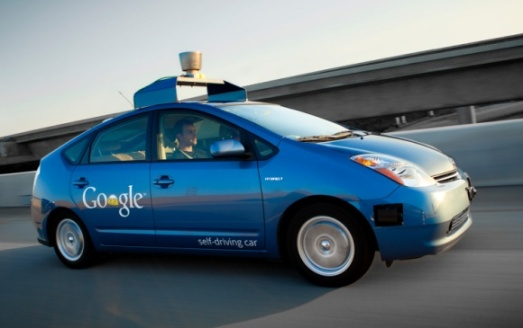
\includegraphics[width=0.4\linewidth, height=5cm]{figures/1-1a.jpg} 
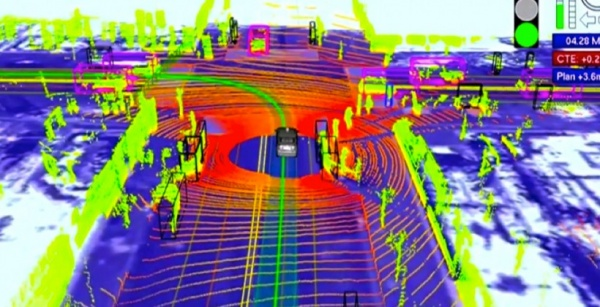
\includegraphics[width=0.4\linewidth, height=5cm]{figures/1-1b.jpg}
\end{center} 
\vspace{-4mm}
\caption{Google自动驾驶汽车和其场景感知的示意} \label{fig_1-1}
\end{figure*}

\begin{figure}[tb]
\begin{center}
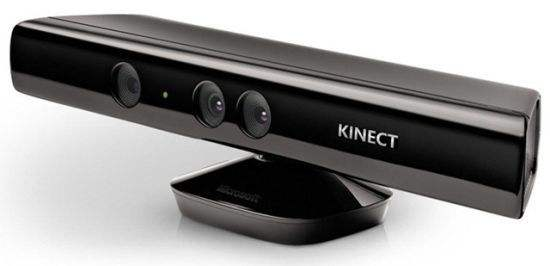
\includegraphics[width=0.4\linewidth]{figures/1-2.jpg} 
\end{center} 
\vspace{-4mm}
\caption{微软发布的首款RGB-D设备Kinect} \label{fig_1-2}
\end{figure}

近年来,业界对三维模型的研究是如火如荼,三维模型因为其丰富的形状、颜色、纹理等信息,在多媒体,图形学,虚拟现实,设计,娱乐,工业制造等领域得到了越来越广泛的应用\cite{Tangelder2008A}。大量的三维模型例如Google3D Warehouse数据库可以从网络上轻松获得。同时3D打印技术的出现,使得三维形状模型的应用更加实用化,这种增材制造技术能够完成许多传统减材制造技术所不能完成的复杂产品生产。除此之外,随着RGB-D设备的出现,如图\ref{fig_1-2},用户可以更加方便快捷的获得三维模型数据,这也大大增加了三维模型的数量。因此,为了有效地对现有三维模型进行高效的管理和再利用,在三维形状的匹配,查找和分类等方面获得优秀的表现,我们需要高效准确的图形检索、分类的方法来处理这些海量三维数据。

三维形状模型与一般的二维图像相比,更丰富真实、更好的符合了人类视觉特性、能够更加清楚的表示现实世界的物体。一般情况下三维形状模型由网格数据结构,包括顶点、面、边等基本数据来表述,因此具有相对复杂的数据结构,与声音、图像相比更加难以处理。目前随着三维扫描技术与设备和交互建模工作的快速发展,使得三维形状模型的数量快速增加,这为许多需要使用3D模型的领域提供了方便。但由于三维模型较其他类型的数据结构相比复杂,目前仍然存在一些难以解决的问题:由于大量的三维模型已经存在,不需要使用者自己亲自去建模型,但如何在大规模的三维模型库中快速并准确地找到自己所需要的模型依然是一个难以克服的问题。另外三维形状匹配还可以在以下领域得到广泛的应用,机器人或无人飞行器通过三维形状匹配在数据库中快速地检索并识别物体,用来寻找并确定目标或者用来躲避障碍物,提高其自身的智能程度;公共安全等领域利用三维匹配技术来查询二维或三维人脸库、三维头颅库等匹配相关信息,能够大大降低恐怖袭击和刑事犯罪对社会的危害;工业现场可以根据图像或图形匹配自动判定控制信息、故障类型等;在生物医学方面,由CT、MRI、PET等断层成像设备产生了大量的三维数据,如何准确快速地查找并处理这些信息,对于提高诊断的准确率并提高我国医疗健康水平,缓解人口老龄化带来的压力至关重要。

对于三维图形的分类和检索,大部分的解决方案都是设计出优秀的三维形状特征。三维形状特征很好地描述了三维模型的相关属性包括颜色、纹理、形状特性等,用于有效的区分或者归类不同的三维模型。目前大量用于描述三维模型的特征被提出,例如:平均测地线距离 (Average Geodesic Distance),尺度不变的热核描述子 (Scale-invariant Heat Kernel Signature),形状直径函数 (Shape Diameter Function)等,尽管这些特征在某些方面取得很好的应用,但是在很多实际应用中还有待进一步提升。主要原因有两点:第一,这些特征都是基于专业的设计人员通过复杂的数学模型构建出来的,需要相关领域很强的先验知识。第二,人工设计的特征大部分只能抽象三维模型上某一方面的属性,而三维形状含有复杂的三维拓扑结构以及丰富的几何信息,很多信息在特征提取完之后严重丢失,从而影响了图形的检索效率。

同时三维形状内容的匹配与检索没有像文本内容匹配与检索那样简单,从一篇文章中提取若干关键文字信息,或从一幅图像、一段视频中提取能够代表该图像的描述信息相比,因为三维形状的数据结构存在拓扑等复杂结构,因此处理相对复杂,已研究出的特征提取、匹配与检索方法仍存在一定的局限性,因此目前只有具有高级思维的人类才可以完全实现。通过计算机提取多媒体信息的特征仍然是一件困难的事情,也是多媒体匹配与检索的核心技术之一\cite{Tangelder2008A, Funkhouser2005Shape}。三维模型匹配、对齐、分割中,形状特征的提取是非常关键的技术之一,提取的形状特征需要有如下特点:1)良好的类间可分性和类内相似性,用以保证形状描述的准确性;2)对形状的变形有较高的鲁棒性,特别是非刚性变形; 3)尽可能低的特征维数,和能够表示三维形状的显著特征,这样就能减少搜索或者匹配的计算量,大大提高计算性能。



\section{三维模型的研究状况}

\subsection{国外现状分析}
国外对三维形状识别研究起步较早,研究者主要关注于整体特征的提取,已经获得了大量的研究成果\cite{Tangelder2008A,Funkhouser2005Shape,Krizhevsky2017ImageNet,Kaick2010A,Ullman1985Three, Loncaric1998A, Campbell2001A}。美国Carnegie Mellon大学的Johnson等人\cite{Johnson2002Using}提出了一种经典的局部描述符 Spin Image,该描述符将临近的顶点投影到了一个二维的柱面坐标下,因此复杂的三维形状匹配转化成了相对简单的二维图像的匹配。该方法具有很强的鲁棒性,但这个方法中需要计算并匹配每个顶点的spin image,因此计算效率不高,此外该特征描述符无法很好的应对非刚性变形。之后美国Sarnoff公司的Shan等人\cite{Shan2006Shapeme}提出了使用Shapeme投影的方法来分割需要匹配的形状,从而加速形状匹配的速度; Liu等人\cite{Liu2006Shape}提出了使用Monte Carlo稀疏采样的方法来降低计算量,并使用k-means方法使得到的数据量得到有效的降低从而提高匹配速度。另外希腊Centre for Research and Technology Hellas的Malassiotis等人\cite{Malassiotis2007Snapshots}提出了Snapshot局部特征描述符,该描述符能够很好应对自身的重叠以及假象的影响,并且该方法使用更高效的特征对齐方法,能够获得很好的性能,但仍然无法很好的应对非刚性变形。

大多数情况下,对象物体不仅仅含有刚性变形,还具有非刚性变形,例如弯曲、姿势改变、局部形状变化等。这种变形过程中任意两点测点距离不变,即称之为等距变形。为了解决前述方法无法应对非刚性变形问题,近年来研究者做出了大量的努力。美国ioIMAGE公司的Elad等人\cite{Elad2001Bending}首先在这方面做了尝试,他们根据形状弯曲变形中表面上的长度并未发生变化这一特点,使用Multidimensional Scaling (MDS)将测地线距离转化成了欧式空间的距离,因此非刚性变形的转化成了简单的刚性形状匹配。之后美国Stanford大学的Emoli等人\cite{M2005A}与以色列的Israel Institute of Technology大学的Bronstein等人\cite{Bronstein2006Efficient}扩展了这项研究,他们使用Gromov-Hausdorff距离来计算形状的相似程度,这样能够有效的降低两个形状建立对应关系时所产生的误差。由于这类方法基于高计算复杂度的最优化方法,因此只能适用于一对一,或者一对少数形状的匹配。德国University of Hannover的Reuter等人\cite{Reuter2006Laplace}提出使用Laplace-Beltrami谱作为等距变形的形状描述符,这个描述符具有更小的计算复杂度,因此最近受到很大的关注。Wu等人\cite{Wu2010Global}扩展了这个方法,在他们的研究中使用随机采点的方法得到一定数量的顶点,在每个顶点附近使用固定面积比率的方式选择一个局部区域,然后计算该局部区域的Laplace-Beltrami谱,然后与全局的Laplace-Beltrami谱进行结合,这样兼顾了全局和局部特征,因此获得了更好的性能。美国Stanford大学的Sun等人\cite{Sun2009A}提出了热核特征(Heat Kernel Signature: HKS)的描述符,通过求解每个顶点的热扩散方程,求取基础解-热核作为局部特征。其优点在于选择不同的扩散时间可以控制所包含的局部范围。该方法只需要特征分解拉普拉斯系数矩阵,效率较高,弱点在于不能应对尺度变换和拉伸变换。以色列的Israel Institute of Technology大学的Bronstein等人\cite{Bronstein2010Scale}改进了热核特征描述符,使之能够应对形状的尺寸变形的影响。

另外一方面,由于三维形状的各个部分的重要程度不同,因此利用区域的重要程度来选择需要匹配的顶点或区域能够极大地降低计算复杂度并提供形状对应、匹配、与检索的速度。首先是美国Maryland大学的Lee等人\cite{Lee2005Mesh}提出了对高斯加权平均曲率做center-surround的网格显著区域提取的方法,通过实验得知该方法能够捕获网格上绝大多数的显著区域,但该方法的缺陷是得到的显著区域过于稀疏,导致形状匹配精度的下降。之后,美国Princeton大学的Shilane等人\cite{Shilane2007Distinctive}提出另一种形状显著区域提取的方法,任意一个给定顶点对已建立的数据库进行检索,使用DCG(discounted cumulative gain)值来衡量该点所覆盖的区域是否为显著区域,若使用该区域检索能够获得高的DCG值,则表明该区域是重要,反之则认为是普通的区域相对不重要。该方法能够提供更高精度的局部显著指标,然而这个方法由于计算量大,并且需要事先构建一个形状数据库,因此比较难以在实际中应用。波兰Institute of Theoretical and Applied informatics of PAS的Glomb\cite{G2009Detection}将图像领域的Harris运算符扩展到了三维领域,通过计算顶点附近区域的形状变化来衡量该点局部区域的显著程度。法国INRIA Grenoble Rhone-Alpes的Zaharescu等人\cite{Zaharescu2009Surface}将图像领域内知名的Difference of Gaussians (DOG)显著区域提取方法扩展到了三维,并提出了Mesh DOG方法,该方法具有对方向、旋转、平移和缩放具有较高的鲁棒性,但仍然不能很好的应对非刚性变形。

由于三维形状的匹配与检索相对复杂,很难推导出理论的评价方程,因此常常使用标准形状库来评价各种方法。美国Princeton大学的Shilane等人\cite{Shilane2004The}提出一套三维模型库Princeton Shape Benchmark,该数据库包含了1814个通用物体模型,并分成了训练和测试两组。加拿大McGill大学Siddiqi等人\cite{Siddiqi2008Retrieving}提出了专门针对关节变形物体的形状标准库McGill 3D Shape Benchmark。以色列Israel Institute of Technology大学的Bronstein等人\cite{Bronstein2009Numerical}设计并制作了专门针对非刚性变形的形状标准库TOSCA,可供部分匹配和检索研究之用。美国国家标准与技术研究院提出的SHREC2011非刚性变形形状库\cite{Lian2011SHREC},包含600个非刚性变形的物体,适合包含非刚性变形方面的分析与评价

\subsection{国内现状分析}

国内在三维形状特征描述符方面起步较晚,研究主要集中在全局特征描述符上,经过近几年的努力取得了可喜的研究成果。韩等人\cite{韩丽2015Laplacian}面向三维模型的统一结构描述与智能检索的技术需求,提出一种Laplacian多特征映射的三维模型形状分析方法。霍等人\cite{霍磊2015基于显著点切片的三维模型检索}提出了使用模型显著点进行切片的方法以及基于点分布和Zernike矩的融合特征提取方法。刘等人\cite{刘志2016基于特征线条的三维模型检索方法}为了避免在三维模型检索中对输入源的限制,提出一种以自然图像为输入源、基于特征线条的三维模型检索方法。黄等人\cite{黄骥2016基于核线性分类分析的三维模型检索算法}为提高检索精确度,提出了一种利用核线性分类分析来对模型特征进行优化的新方法。屠等人\cite{屠宏2015一种基于局部特征的三维模型检索算法}面向在基于内容的三维模型检索系统中,特征提取技术是三维模型检索的关键的需求,提出了基于局部特征的三维模型检索算法。张等人\cite{张全贵2017融合}针对手绘草图检索三维模型时存在的表达模糊性和绘制随意性等问题,提出基于Fuzzy拓扑关系与角点典型形状上下文(CRSC)的三维模型检索方法。周等人\cite{周燕2016基于多特征融合的三维模型检索算法}针对三维模型检索中单一特征检索效果差的难题,首先提出了三维模型的3类特征向量提取算法,即刻画模型表面特性的扩展高斯球面特征向量、反映模型内部结构的Radon变换球面分布特征向量、代表模型投影层次的视图分层压缩感知特征向量。其次,以样本模型的查询结果分类信息熵作为指标并结合监督学习过程,给出了一种多特征融合的加权系数估算方法。计等人\cite{计明明2015基于多特征融合的三维模型检索技术}提出一种基于多特征融合的三维模型检索框架。朱等人\cite{朱新懿2015使用形状变化描述三维模型}针对三维模型检索中的形状特征提取问题,提出利用三维模型自身形状变化信息构造形状特征描述符的方法。李等人\cite{李闯2016基于平均自旋图的三维形状特征描述}基于自旋坐标和自旋图理论,给出基于平均自旋图的三维形状特征描述方法,用于三维模型检索。王等人\cite{王新颖2015基于异构特征}提出一种包含语义分类信息的三维模型检索方法。采用人工分类信息、有限的语义标准信息等构建异构语义信息网络,并将其转换为三维模型的异构语义特征,在此基础上使用包含模型语义特征的主题分类方法,并将其应用于模型检索中。徐等人\cite{徐平安2015融合细节与整体特征的三维模型检索方法}提出一种融合细节与整体特征的三维模型检索方法,通过 SIFT 特征和傅立叶描述子特征来对三维模型进行特征描述。肖\cite{肖秦琨2015融合深度图和三维模型的人体运动捕获}等人提出了一种融合深度图和三维模型的人体运动捕获方法。利用Kinect采集深度图像,经过对深度图去除背景,提取轮廓信息,建立轮廓数据库。从深度图中提取三维人体骨架, 建立骨架三维模型数据库。侯等人\cite{侯晓丽2014基于局部特征的图像匹配算法研究}通过对经典的图像匹配算法,特别是基于特征匹配的SIFT和MROGH算法的研究提出了基于环状划分的局部坐标系特征描述的图像匹配算法和基于颜色不变量的局部特征图像匹配算法。阮等人\cite{阮孟贵2010基于图像三维模型重建的研究}提出了立体视觉方法采用动态规划方法进行匹配获得对应象素的视差,并通过三角测量原理获得深度信息和一种快速的基于轮廓的三维模型重建方法,将传统三维锥形交叉问题转换成二维轮廓交叉问题。

\section{深度学习技术}

深度学习(Deep Learning)发展于上世纪末,其是由神经网络发展而来。由于其出色的表现,逐渐使得其成为研究的热点。针对深层次网络训练的难题,人们提出了BP算法\cite{Rumelhart1988Learning}。BP算法是深度学习的基础算法之一。Yann LeCun等\cite{Lecun2014Backpropagation}提出了卷积神经网络(Convolutional Neural Network)是深度学习技术的一次成功应用。然而,能够训练的网络深度只有两到三层,严重抑制了深度学习的发展进步。事情的转机出现在2006年,Hinton等人\cite{Hinton2006A}提出了深度置信网络模型(DBN),并给出了一种自底向上对网络参数进行逐层预训练的贪婪算法,这种方法每次只训练网络结构中的一层,然后利用有标签的数据对参数进行微调,这种方法可以有效地对多层的前馈网络模型进行预训练,深度学习的概念由此诞生。
%
随着深度学习技术不断发展,大量的新的深度学习算法被提出。其中比较出色的包括自动编码器(AutoEncoder)、卷积神经网络(CNN)、循环神经网络(RNN)、深度神经网络(DNN)、深度玻尔兹曼机(DBM)、卷积深度置信网络(CDBN)等等。2012年,Alex等人利用卷积神经网络设计的算法在Imagenet图像识别竞赛中取得了巨大的突破\cite{Krizhevsky2017ImageNet},在后续图像各方面的研究中,这种类型的卷积神经网络都已经被广泛采用。而在声音识别领域,百度公司采用深度学习方法研发出的语音识别系统Deep Speech,即使在各种复杂的环境中,也能取得非常好的识别效果\cite{Niu2014Context}。在自然语言处理领域,另一种网络结构形式的深度学习模型RNN,已应经在机器翻译、文本解析等方面取得了非常大的进展。

近年随着深度学习算法的深入研究,深度学习算法已经深入到IT领域的各个方面,各个互联网巨头都不惜重金,发展深度学习,例如腾讯的DX-I框架,阿里巴巴的PAI2.0框架。Google的Deepmind团队的AlphaGo更是在围棋方面战胜世界一流棋手李世石。不久前更是推出了``最强版”AlphaGo Zero。深度学习已经是当前计算机技术的风口浪尖,其能够通过学习的方式得到表达能力更强的阶层式特征,并对海量数据进行处理,因此深度学习的方法可以应用于三维形状的识别问题。一般的特征包括颜色的直方图,纹理的直方图,Gist,HoG, SIFT, SURF等,尽管这些特征在某些应用中取得了比较理想的效果,但是它们只能刻画图像当中某一方面的信息,也就是说这些特征在不同的任务中,效果并不都是最优的。
%
最近几年越来越多的研究表明,特征的提取和分类是相互交织在一起的,通过学习方式得到的特征能够获得更高的性能。图像信息在人类理解和认知外界环境中起到主要的作用,将图像信号经过人脑视觉系统处理之后,我们能够对物体进行识别、对场景进行理解,从而使得我们能够对环境做出反应。但是,为什么人脑有如此强大的信息处理能力,从而让我们在短时间之内对环境做出非常准确的理解与判断?以及怎样才能让机器模拟人的大脑视觉系统处理图像?神经生物学家、生物医学家对人脑进行研究发现大脑的视觉系统处理是一种“分层学习” 机制,如图\ref{fig_brain}所示。

\begin{figure}[tb]
\begin{center}
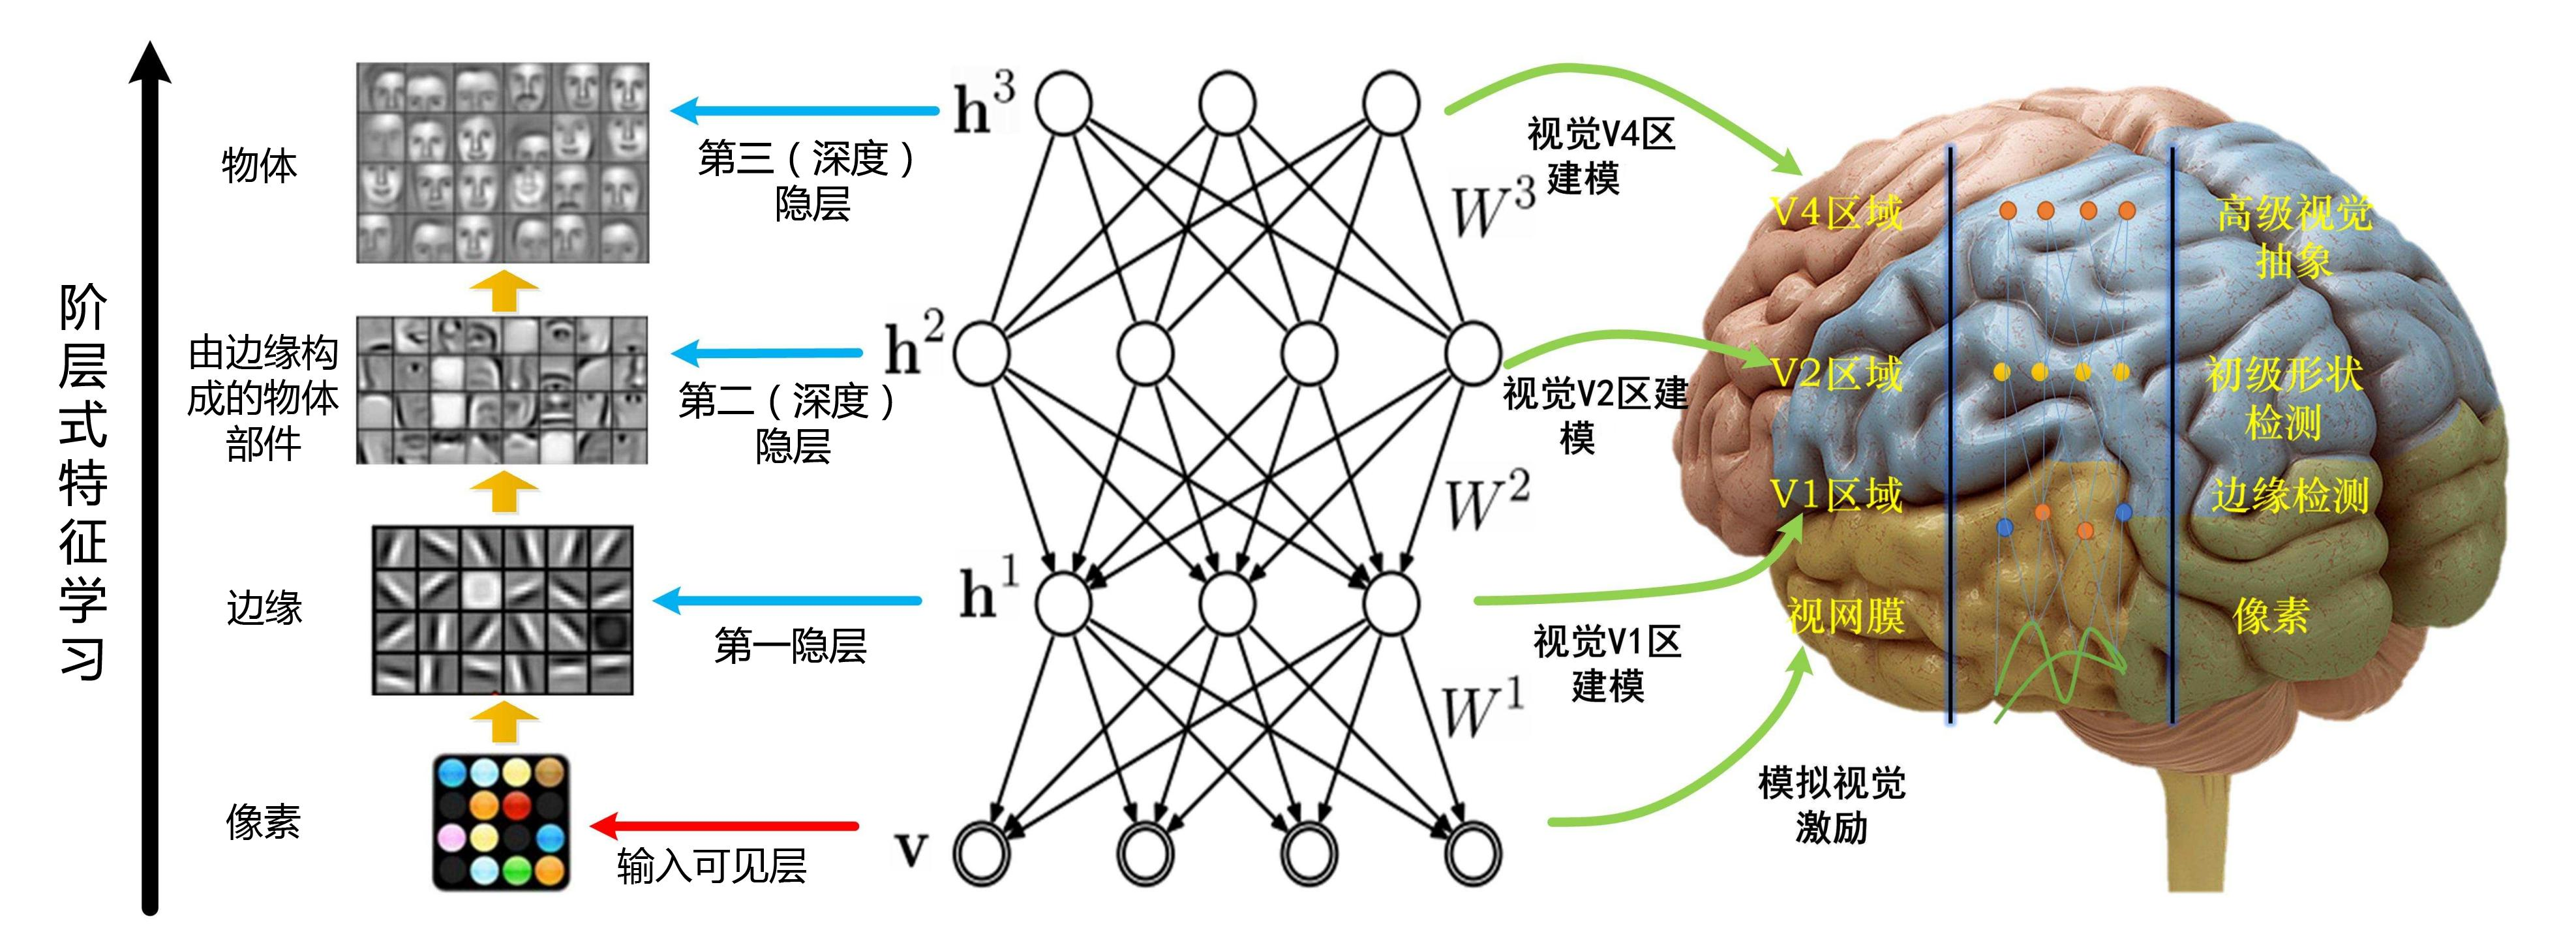
\includegraphics[width=0.9\linewidth]{figures/1-3.jpg} 
\end{center} 
\vspace{-4mm}
\caption{大脑认知和深度学习的关系(示意图)} \label{fig_brain}
\end{figure}

从原始信号摄入开始(瞳孔摄入的图像),接着做初步的处理(图像中的边缘等),然后抽象(眼前的物体是嘴或者眼睛),然后进一步分析(该目标是一个人脸)。人类的这种分级认知机制,从机器处理图像的角度来看是一种从低级特征提取到高层特征提取的过程。因此,实现机器像人类一样认知三维形状,图像的特征提取至关重要。如果想要模拟人类视觉系统的分层学习机制,则需要经验丰富的算法设计工程师根据不同的需求,设计出不同层次的特征提取方法,工作量很大并且缺少通用能力。

另一方面,在机器学习领域,目前常用的学习算法例如支持向量机、提升算法,普通的神经网络等都是浅层模型,这些方法的模型通常只有1-3个信息处理层,无法处理现实世界的高度复杂的非线性数据;而人类的大脑的认识、学习是通过多层次的处理来实现的,从而使解决问题的规模可以非常庞大。最近十年间,由于新的神经网络学习方法的研究和计算机能力的提高,克服了以往神经网络层数多而导致的无法训练、过拟合等问题,从而使深度学习得到了快速的发展。最新的研究成果表明,通过深度学习,能够让计算机生成较高层次的语义信息,因此能够填补底层特征和高层语义之间的鸿沟,所以能够极大地提升人工智能的程度。

深度学习已广泛应用于自然语言处理,语音识别,计算机视觉等诸多领域,并展示出了非常优异的性能\cite{Krizhevsky2017ImageNet, He2015Delving, Mnih2015Human}。Dahl等人\cite{Dahl2012Context}提出了一种融合隐马尔科夫模型的混合深度网络并应用于语音识别,在非常具有挑战的数据库上获得了理想的识别精度。Lee等人\cite{Honglak2009Convolutional}使用了卷积深度置信网络来提取图像的阶层特征,在几个图像数据库上都获得较好的识别率。Nitish等人\cite{Srivastava2012Multimodal}提出了多模态的深度学习方法,他们使用了两个深度置信网络来对图像数据和文本标签数据进行建模,并在两个深度网络的上层构建了一个联合表达层来表达这两种数据的关联性。与传统的支持向量机方法相比,该方法能够充分利用多种来源的信息,因此能够获得更高的性能。Kae等人\cite{Kae2013Augmenting}提出了一种融合CRF和玻尔兹曼机的图像标签方法,通过这种融合使深度学习方法提高了结构学习能力。

\section{论文的研究内容及贡献}
目前深度学习(Deep Learning, DL)已经广泛应用于各个领域,可是在三维形状领域目前还不成熟。对三维形状识别检索领域的不断探索,能够不断拓宽深度学习在三维形状分析领域的应用,不断提高三维形状的识别精度,使其更好的服务于社会生产中去。具体来说,论文的贡献如下:

\begin{itemize}
\item 结合多模态融合的思想,首次提出了结合CNN、CDBN、DBN、RBM的多层神经网络的多模态信息融合方法,从而得到具有强表达性质的三维形状特征。
\item 提出了利用获取三维形状视觉信息具有序列化时空信息,提出了基于CNN、LSTM的三维形状识别方法
\end{itemize} 

\section{论文结构安排}

第一章绪论部分介绍了本文的研究背景及意义,说明了本文的研究内容和主要贡献。

第二章详细分析了目前深度学习技术在三维形状应用的最新进展。

第三章详细介绍结合CNN、CDBN、DBN、RBM的多层神经网络的多模态信息融合方法。

第四章详细介绍了基于CNN、LSTM的三维形状识别方法。

第五章对本文工作做了总结,并对后续工作进行了展望。

% \begin{table}[h]
%     \caption{测试运行环境}
%     \centering
%     \begin{tabular}{ccc}
%         \toprule
%         操作系统    & \TeX 系统   & 版本 \\
%         \midrule
%         Windows 10  & TeXLive     & 2013 \\
%         CentOS 7    & TeXLive     & 2015 \\
%         \bottomrule
%     \end{tabular}
% \end{table}



\chapter{深度学习在三维形状分析领域的进展}

随着深度学习的不断发展,不仅在计算机视觉方向取得了巨大成功,而且也被广泛应用于三维形状领域,并且取得了一定的成绩。由于三维形状复杂的拓扑结构和丰富的几何信息,如何将深度学习成功的应用于三维形状领域是一大挑战。为了解决三维形状的识别和检索任务,研究人员们主要沿着如下五个不同的方向进行研究。
\begin{enumerate}
\item 从三维形状中提取描述特征,将其作为深度神经网络的输入,进行学习。
\item 利用目前流行的低成本的RGB-D相机(如微软的Kinect)捕获RGB-D信息,将其作为深度神经网络的输入特征。
\item 直接作用于3D数据的深度神经网络,学习3D形状特征。
\item 利用从不同角度观察三维形状得到的二维图,将三维问题转化为二维问题,之后再利用深度学习方法得到高效的、鲁棒性强的三维形状特征。
\item 深度神经网络作用于超光谱相机拍摄的3D数据。
\end{enumerate}

\section{DL作用于三维模型低层特征}

三维模型低层特征描述符常常被用来进行3D数据的识别检索任务。然而,在三维领域中,由于三维数据的复杂性,通常需要高效率的三维形状描述符。通常的做法是提取的低级别的描述符,之后将他们作为深度神经网络(DNN)的输入,从而使识别和检索任务能有高层次的表现。
\begin{figure}[tb]
\begin{center}
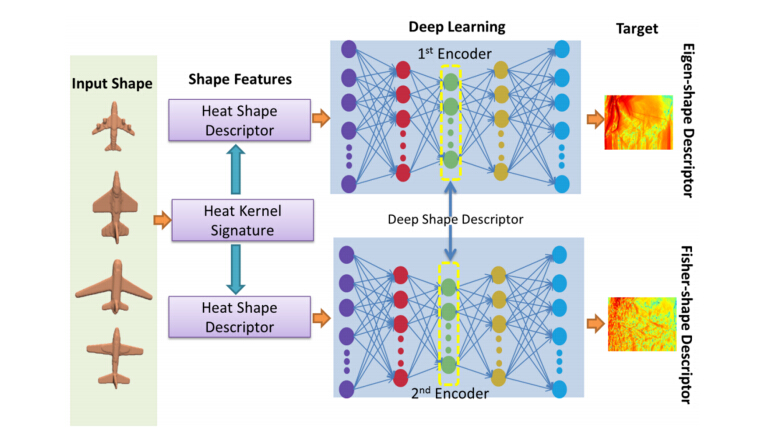
\includegraphics[width=0.9\linewidth]{figures/Fang.jpg} 
\end{center} 
\vspace{-4mm}
\caption{Fang等人提出的三维深度形状特征描述子} 
\label{fig_Fang}
\end{figure}

Liu等人\cite{Liu2014High}采用了深度置信网络(DBN)进行学习3D数据的训练学习,他们采用来自3D数据的底层特征作为DBN的输入数据。具体来说,首先获取每个3D形状的200张深度图像,然后提取每张深度图的SIFT特征描述子。之后,构建BOW字包模型,其中SIFT描述子被编码成BOW模型的``单词''。这些来自三维模型的BOW特征向量,作为DBN的输入数据,对DBN进行逐层的贪婪算法的训练,得到高表达能力的3D特征描述子。该实验同时进行了3D形状的分类和检索实验。实验结果表明该方法获得了比标准BOW模型更为优秀的表现效果,同时证明了在3D数据分析领域深度学习技术具有优秀的效果,并能产生高水平的特征描述子。Bu等人\cite{Bu2014Learning}所作的工作是结合Scale Invariant Heat Kernel Signature (SI-HKS) 和 Average Geodesic Distance (AGD)这两种来自3D数据的局部特征描述子,组成一个低层的3D特征,该特征是由SI-HKS的前6个频率分量和AGD值组成的。接着,一个被称做Geodesics-Aware Bag-of-Features (GA-BoF)的BOW模型的变种被生成。接下来,从GA-BOF中获得的中层特征描述子被用来训练DBN模型,其中DBN的训练采用对比散度的方法。从DBN出来便得到了高层特征描述子。对于3D数据的分类实验中,DBN被认为是一种降维方法,因此他们比较了类似的降维方法,像Principal Component Analysis (PCA) 和 Multi-Dimensional Scaling (MDS)。对于3D模型的检索实验中,DBN模型对比了一些常见的3D数据特征描述子,像Heat Kernel Signature (HKS)。实验结果表明高层特征描述子相较于常见的特征描述子具有更好的可区分性,增强了分类与检索效果。这些被DBN生成的高层特征描述符,又被称做局部深度特征(Local Deep Feature)。在之后的相关工作中,Bu等人利用了基于GPU的深度学习工具包,加快了整个算法的运行速度。

Xie等人\cite{Xie2015Deepshape}将3D形状在不同尺度下的Heat Kernel Signature(HKS)的分布提取出来,用作3D数据的低层特征描述子。这个多尺度的分布特征被用来作为AutoEncoder(AE)深度网络模型的输入,从而获取高层特征描述子。为了提高特征描述子的判别能力,采用了Fisher判别准则。该三维数据的特征表达是由AE的所有激活状态的隐层链接而成。三维形状的匹配和检索实验表明,该高层特征描述子具有鲁棒性对变形不敏感。2015年,Fang等人\cite{Fang20153D}提出了类似的深度学习框架,作者提出的深层三维形状描述符,是利用Heat Shape Descriptor(HeatSD)的方法,该方法是由基于HKS的不同尺度下的形状描述子和多对一的编码器构成。多对一编码器确保了完全相同的输出是由相同类的输入产生。主成分分析(PCA)和线性判别分析(LDA)分别被应用于提取三维模型的HeatSDs来生成特征形状描述符Eigen-Shape Descriptor(ESD)和Fisher的形状描述符(FSD)。预先计算的ESDs和FSDs被作为目标值,分别用来训练两个独立的编码器。该方法同时最大化了类间的边缘和最小化了类内的方差,提高了深度形状特征描述子的判别能力。整个流程图如图\ref{fig_Fang}所示,三维形状特征描述子子在三维形状检索中取得了良好的效果。

\section{DL作用于RGB-D数据}

随着RGB-D传感器逐渐普及,像微软的Kinect传感器,人们可以轻易的获得大量的三维形状的RGB-D数据。这种传感器除了提供常见的RGB三通道的颜色信息外,还提供了额外的深度信息,因此许多研究工作利用这些来自三维模型的RGB-D信息处理诸如3D形状识别、检索和语义分割等信息\cite{Sanchez2016A}。

Socher等人\cite{Socher2012Convolutional}首先提出了基于RGB-D数据对三位形状进行分类的方法。他提出的方法是将卷积和递归神经网络(recursive neural networks)相结合,分别对颜色信息和深度信息进行独立处理。具体来说,首先,利用两个单层的CNNs分别提取RGB图像和深度图像的低层特征描述子。然后,不同的CNNs的输出被输入到不同的RNN模型中去,其中模型的所有权重都是随即初始化的。从RNN中得到的每一个特征最终被合并成一个特征,同时将其带入到一个联合的softmax分类器中。该方法在对家庭中的三维形状分析中具有精确的性能。Couprie等人\cite{Couprie2013Indoor}采用了多尺度的CNN用来对室内的RGB-D场景进行语义分割。该网络能够处理三个不同尺度的深度图像和RGB图像,然后这些分别得到的上采样结果被合并成一个特征,之后被带入到分类器中从而得到分类标签。最终的分类标签同时融合了分类器的预测结果和RGB-D场景的超像素分割的结果。实验表明,这种方法比在这之前的方法更加有效,运行速度更快。Alexandre\cite{Alexandre20123D}探索了在CNNs之间使用迁移学习用来对3D模型进行识别的可能。该方法应用了四个独立的CNN处理RGB-D图像的四个独立的通道信息。四个CNN依次的进行训练,其中将上一个训练好的CNN权重作为下一个CNN的输入。10个类别的3D物体的实验表明,所提出的训练策略可以提高三维形状分析性能。

在Schwarz等人\cite{Schwarz2015RGB}的基于深度CNN网络的迁移学习也是致力于解决RGB-D物体的识别。其架构采用了一个预训练的CNN进行图像分类,同时将颜色和深度信息分开作为输入对CNN进行训练。这些输入数据进行必要的预处理,以便将他们转换成适当的格式。Schwarz认为深度信息方面,应该从一个规范的视角来渲染物体,同时根据据物体中心不同的距离来对深度进行着色。实验使用网络的最后两个FC层的输出作为描述符,而SVMs最终被用来预测被测试对象的类别、实例和姿态。Eitel等人\cite{Eitel2015Multimodal}也提出了解决RGB-D物体识别的方法。其设计了一个两流CNN结构用来RGB-D物体的识别任务。这两个流(一个用于颜色,另一个用于深度)包含五个卷积和两个FC层。两流原本单独训练,随后,他们在之后的FC层和softmax分类器中被融合。 由于用来完成识别任务的两个CNNs的需要预训练才能完成基于ImageNet数据集的物体识别任务,因此对输入数据进行预处理,尤其是深度信息的处理,是非常必要的。像这种将深度信息编码成彩色图像的方法,被实验证明,效果优于当时其他现存方法。此外,一种新的数据增强方案被采用,该方案生成人工噪声模式,并将它们用作额外的训练样本。大量的实验结果表明,所提出的方法在真实场景、噪声场景中的目标识别任务中具有很好的性能。 Feng等人\cite{Feng20163D}提出了一个集成的CAES(如图\ref{fig_Feng}),利用从类似Kinect的相机获取的一张深度图来解决三维形状的检索问题。每个AE都使用SDG在不同的数据库CAD模型上进行训练。由于该查询不同的数据类型(例如,深度数据)对训练数据的比较(例如CAD模型),所有的AES输出结果转发到一个新的层,称为域适应层(DAL),以确定检索排行。实验结果表明,与其他相关方法相比,该方法获得了更好的性能,比如方向梯度直方图(HOG)描述子,使用L2范数或全局AE。 

\begin{figure}[tb]
\begin{center}
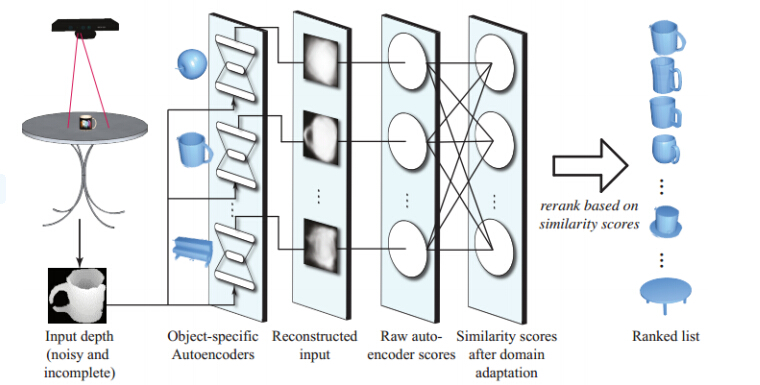
\includegraphics[width=0.9\linewidth]{figures/Feng.jpg} 
\end{center} 
\vspace{-4mm}
\caption{基于深度的压缩自编码器的检索框架} 
\label{fig_Feng}
\end{figure}

\section{DNN直接作用于3D数据}
在过去的几年中,利用捕获场景的完整三维几何图形直接作为DNN的输入的方法已经开始出现。Wu等人\cite{Wu20143D}提出了一种利用整个三维结构实现三维形状表征的新方法。该方法被称为3D ShapeNets,其基本结构为以三维形状作为深度神经网络的输入。这种输入是三维体素网格,这是一种二进制表达,即就是我们认为某个体素网格是否属于该三位形状的一部分。这种体素网格作为之后的DBN的输入,进行训练学习。为了减少与正常分辨率的三维体素量进行全连接时,DBN所需参数数量巨大,于是采用了三维滤波器卷积来降低参数数量。最特别的是,其提出了卷积深度信念网络(CDBN),CDBN一共包含五层,其中三层卷积,一个完全连接层,和一个输出层。该模型首先进行逐层初始化,之后,通过反向传播算法进行微调。标准对比散度被用来训练网络前四层,但更复杂的快速持续对比散度(FPCD)被用于训练网络的顶层。该框架在被用在多种任务,例如三维形状的分类和检索,下一个最好视角预测和基于视图的2.5D的识别任务,在这些任务中都表现优异的效果。此外,作者还发布了ModelNet数据集,这是一个全新的大尺度三维数据集,包括662个不同类型的CAD模型。

Maturana和Scherer\cite{Maturana2015VoxNet}也尝试了使用三维数据的空间表达式进行三维模型的识别方法。如图\ref{fig_Maturana}所示,该VoxNet框架是由体积大小为32×32×32体素网格,该体素网格产生于点云的分割之中,之后将其作为CNN的输入进行训练。该网络架构是由两个带有3D滤波器的卷积,一个池化层和两个全链接(FC)层构成,采用带有动量的随即梯度下降(SGD)的算法进行训练。每一个点云的分割部分,被预测得到一个预测标签。
\begin{figure}[tb]
\begin{center}
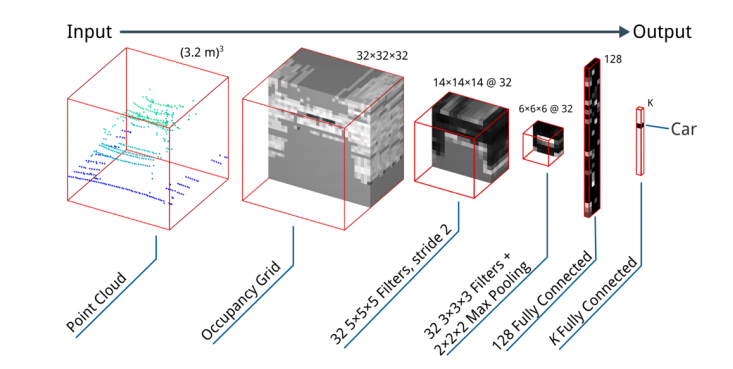
\includegraphics[width=0.9\linewidth]{figures/Maturana.jpg} 
\end{center} 
\vspace{-4mm}
\caption{三维模型的识别的VoxNet4架构} 
\label{fig_Maturana}
\end{figure}
Maturana采用了三个不同领域的三维数据,分别是激光雷达点云数据,RGB-D点云数据和CAD模型,来评价VoxNet模型。实验表明,所提出的框架结构比同类方法具有更好的分类精度,同时具有实时性能。具体来说,VoxNet的性能表现优于3D ShapeNets\cite{Wu20143D}在三维形状分类的任务中。该实验所采用的数据集是ModelNet10, ModelNet40和NYU v2\cite{Silberman2012Indoor}。另一方面,当使用ModelNet10预训练的模型时,3D ShapeNets在NYU v2数据集上表现更好。 Sedaghat等人\cite{Sedaghat2016Orientation}修改了VoxNet的架构,以便将模型的方向性考虑进去。在最后的模型中,类标签直接从激活的方形中得到。 该方法改进了ModelNet10和其他数据集的分类结果。

Wang等人\cite{Wang2016An}最近提出了一种新的3D描述符学习方法,即卷积自动编码器极限学习机(Convolutional AutoEncoder Extreme Learning Machine, CAE-ELM)。其结合了CNNs, AEs和ELMs的优势。极限学习机(ELM)是Huang等人\cite{Huang2006Extreme}提出的只包含一个隐藏层的前馈网络。ELM的隐含层实际上是固定的和随机的,而输出层是根据感兴趣的任务以监督的方式训练的。Kasun等人\cite{Kasun2013Repre}提出了具有多隐层的标准ELM模型的深入扩展。Wang等人\cite{Wang2016An}提出的架构包括以下几个部分:(i)卷积特征图生成:在这部分网络中,计算三维输入数据(即体素和有符号距离场(SDF)数据)与随机生成的三维内核和卷积特征地图。接下来,为了保持旋转不变性,对特征图应用平均池化。(ii)AE描述符提取:池化之后,每个特征图被作为输入提供给单独的AE。所有的AE最初都是用随机权重初始化的,最后的(输出)权重是通过训练学习的。(iii)ELM分类器:在网络的最后部分,从AE提取的所有描述符被连接成用于预测当前3D形状的标签的矢量。在三维模型分类,三维形状检索和三维形状完成的背景下,CAE-ELM在ModelNet上进行了测试,与Wu等人\cite{Wu20143D}和Xie等人\cite{Xie2015Deepshape}的方法相比,取得了优势。实验中使用的最终体系结构包括两个平行的CAE-ELM层,一个在体素上,另一个在SDF数据上。Han等人\cite{Han2016Mesh}提出了用于从3D网格学习高判别性3D特征的网格卷积限制玻尔兹曼机器(Mesh Convolutional Restricted Boltzmann Machines, MCRBM)。学习得到的特征保留了局部区域之间的结构关系,同时也可以保留局部与全局之间的结构关系。该结构提供了局部区域的新的原始表示,称为局部函数能量分布(Local Function Energy Distribution, LFED),作为对网络的输入。另外,将多个MCRBM组合起来,形成一个更深的模型,命名为网格卷积深度置信网络(Mesh Convolutional Deep Belief Network, MCDBN)。这两种深度模型在进行了全局和局部形状检索和形状对应的情况下,表现了优于诸如BOW,Chen等人\cite{Chen2003On},Kazhdan等人\cite{Kazhdan2003Rotation},Bronstein and Kokkinos等人\cite{Bronstein2010Scale}和Wu等人\cite{Wu20143D}的方法

Qi等人\cite{Qi2016Volumetric}在开创性的工作中,详细阐述了影响体积CNN性能的两个因素,即网络体系结构和体积分辨率,并提出了两种新的CNN体​​系结构,这些体系结构改善了目标分类当前的最新性能,即VoxNet\cite{Maturana2015VoxNet}平均课程准确率达到83%。Lin等人\cite{Lin2013Network}第一个提出的CNN包括的mlpconv层的3D扩展工作,并试图通过包括对对象的部分进行分类的附加学习任务来强调3D物体的细节。这个网络达到了86%的平均分类准确度。第二个CNN最初利用长各向异性核来考虑长距离相互作用,并开发了一个适应性的NIN网络\cite{Lin2013Network}进行分类,平均分类准确率为85.6%。在这两个网络中,还通过应用几个方位角和高程旋转来训练数据增强,同时还使用了多方位池化,从而进一步提高了性能。广泛的实验评估强调了三维分辨率在体积CNN中的重要性。最近,Brock等人\cite{Brock2016Generative}提出了用于形状建模和3D形状分类的基于体素的(全3D)模型,并且与迄今为止提出的任何其他3D或多视图深度学习方法相比,ModelNet10和ModelNet40的大量分类结果得到改善。作者利用了DNN领域的最新进展,并设计了一种网络模型,其依赖于(i)初始式模块的结构\cite{Szegedy2016Inception}(ii)批量标准化\cite{Ioffe2015Batch}(iii)预先激活的剩余联系\cite{He2016Identity}和(iv)随机网络深度\cite{Huang2016Deep}。所提出的模型Voxception-ResNet(VRN)是45层深。作者使用整合VRN模型得到了ModelNet40和ModelNet10的最新分类结果。 应该指出的是,训练如此深的模型需要大量的数据增强。

Song和Xiao\cite{Song2015Deep}提出了一种用于在RGB-D场景中进行3D对象检测和识别的流程,称为Deep Sliding Shapes。有趣的是,Song和Xiao不是使用了深度通道,而是通过使用定向截断有符号距离函数(TSDF)将每个深度图像转换为完整的三维体素网格来利用场景的原始3D信息。然后利用被称为3D区域建议网络(RPN)的完全3D卷积网络,以从两个不同尺度的3D体素网格生成3D对象边界框,以便能够处理不同的对象尺寸。同时还为每个生成的建议对象提议提供了对象分数。此外,每个检测到的3D建议框及其对应的2D色块(即,3D建议框的2D投影)分别被馈送到3D ConvNet和2D ConvNet,以便同时学习物体的类别和3D框回归。对于建议目标评估,所提出的方法表现出优于最先进的选择性搜索方法(Selective Search method)\cite{Uijlings2013Selective}的3D版本,而“深度滑动形状”\cite{Song2015Deep}的目标检测任务与其“非深度”版本相比较,即手工描述符的3D滑动形状\cite{Song2014Sliding}和带有ConvNets描述符的最先进的2D Depth-RCNN\cite{Gupta2014Learning},具有较为优异的性能。


\section{DL直接作用于3D模型的2D投影/视图}
为了表达3D形状/模型而从不同方向采集的多个2D投影是三维形状分析和理解通常采用的“技巧”。Zhu等人\cite{}通过投影到二维空间来构建3D形状的深度学习的框架,是类似的最早的方法之一。在前面提到的工作中,为了在3D形状检索的应用场景中生成3D形状的全局深度表示,使用了AE。对每个三维模型在位移和尺度方面进行姿态归一化,随后收集他们的一系列二维投影。在用投影预先训练堆叠的RBM之后,使用反向传播对AE进行微调以最小化重建误差。最后,隐藏层用于表示检索过程中3D形状的相应投影/视图。由于每个模型生成不止一个编码(每个投影一个),所以使用Hausdorff距离的变体来计算两个不同3D形状的最终表示之间的距离。实验是在两个流行的数据集进行的,即普林斯顿形状基准(PSB)\cite{}和工程形状基准(ESB)\cite{}。结果表明所提出的架构与其他基于全局描述符的方法LFD\cite{}相比表现更好。此外,基于SIFT的BoW这种全局特征与局部特征的线性组合,是性能有所提升。

Leng等人\cite{}利用自编码器实现了三维形状检索的工作。在其工作中,提出了从CNN启发的标准AE的扩展,称为堆叠局部卷积自动编码器(Stacked Local Convolutional AutoEncoder, SLCAE)。局部卷积自动编码器(LCAE)通过使用卷积运算将局部连接的层代替标准AE的FC层而构建。在LCAE的堆叠版本中,许多编码器被放置在彼此的顶部,并且最后一个的输出被用作三维模型的表示。提供给所提出的AE的输入是三维形状的多个视图的多个深度图像,而该架构的每一层都是使用梯度下降法来训练的。堆叠局部卷积自动编码器(SLCAE)与其他优秀的方法在三个三维形状数据集上进行比较,获得了更好的结果。这三个三维形状数据集分别是PSB\cite{}, 台湾大学数据集(NTU)\cite{}, SHREC'09\cite{}。另外一个叫做3D卷积神经网络(3DCNN)的架构是由Leng等人提出的\cite{}用于同时处理3D对象的多个2D视图。每个形状的视图在被馈送到网络之前被分类成三个合理的序列,以使视图以固定的顺序被列出。3DCNN由四个卷积层,三个子采样层和两个FC层组成。 卷积层最初是以训练AE的相同方式预训练的。之后,整个网络使用反向传播进行了微调。第一个FC层的输出被用作检索的输入数据的表示。对三个数据集(即PSB,NTU,SHREC'09)的评估表明,与其他最先进的方法相比,所提出的方法具有显着的性能。尽管3DCNN表示虽然取得了良好的结果,但是与使用SLCAE获得的检索性能相比,在所所使用的3个数据集中其性能性能偏低,这表明后者的表示可能是一个更好的选择来处理三维形状的检索工作。
\begin{figure}[tb]
\begin{center}
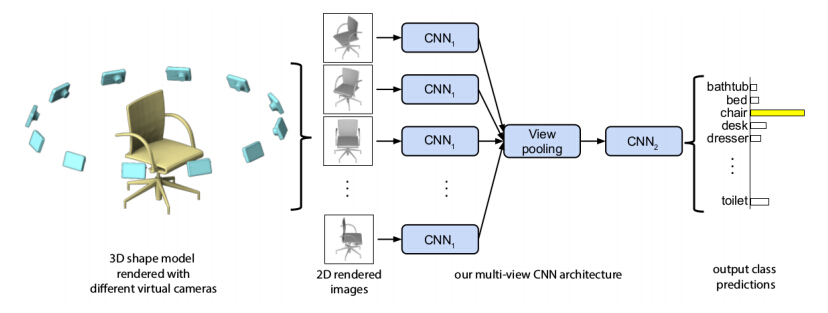
\includegraphics[width=0.9\linewidth]{figures/Su.jpg} 
\end{center} 
\vspace{-4mm}
\caption{MVCNN用于3D对象分类和检索} 
\label{fig_Su}
\end{figure}


Su等人\cite{}的工作也利用了3D对象的多个视图建立一个紧凑的三维物体分类和检索任务的形状描述符。图\ref{fig_Su}所示的新型多视图CNN(MVCNN)体系结构学习了通过视图池化层将任意数量的对象输入视图组合成一个没有特定顺序的视图。为了获得不同的模型的视图,进行了两步设置。第一个设置包括通过在它们周围放置相同数量的虚拟相机来渲染3D形状得到12个视图,而第二个得到80个视图。三维模型的所有可用视图分别通过网络的第一部分,然后在视图池中的所有视图上执行元素最大池化。最后,汇总的结果通过剩余的网络传递。为了检索,网络倒数第二层(完全连接)被用作形状描述符。在MVCNN架构的实验性评估中,网络使用ImageNet1K数据集进行预训练,然后使用3D数据集ModelNet40进行微调。有关形状分类和检索的报告结果显示MVCNN优于所有其他测试方法。值得注意的是,所提出的形状描述符大大超过了Wu等人最先进的3D ShapeNets的性能,特别是在使用ModelNet40数据集的检索任务中。Johns等人\cite{}采用了一种不同的方法来开发3D对象的多个视图针对多视点物体识别在无约束摄像机轨迹下的应用场景。在这项工作中,收集的s视图是组织成对,将他们的相对姿势提供给一个CNN。VGG-M网络\cite{}在这种情况下被使用由五个卷积和三个FC层组成。灰度图像,深度图像或二者同时都可以作为网络的输入。结合来自两个图像的卷积层的输出,之后提供给第一FC层。在ModelNet数据集\cite{}的实验中,这种模型超过了基于体素的3D ShapeNets的性能和Su等人的MVCNN方法。

Bai等人\cite{}提出了一种基于3D对象二维视图的实时三维形状搜索引擎。所提出的系统名为GIFT,利用GPU进行基于CNN的特征提取,并利用两个倒排文件,即一个用于加速多视点匹配过程,另一个用于重新排序初始结果。一个查询形状的检索过程能够在一秒钟内完成。作者在ModelNet、 SHREC14LSGTB\cite{}、PSB、 McGill\cite{}、SHREC'07\cite{}数据集上测试了他们的引擎,均说明了GIFT性能优于较为先进的方法,例如Chen等人\cite{}、Kazhdan等人\cite{}、Wu等人\cite{}和Su等人\cite{}的方法。Wang等人\cite{}最近提出了一种基于二维草图和二维视图检索三维模型的不同方法。更具体地说,Wang等人提出了一个体系结构,输入是一个对象的{2D视图+草图}对。该模型由两个连体CNN(即两个相同的子卷积网络)组成,一个用于处理要被检索的3D对象的2D草图,另一个用2D视图处理。两个子网分别使用SGD和反向传播进行训练。









\chapter{实现}

\section{思路}
\section{代码}


\backmatter
\bibliographystyle{nputhesis}
\bibliography{ref}

\Appendix
This is appendix.

\Thanks
This is a thanks.

\Work
% TODO 如何直接引用使参考文献的内容显示在这里

\statement
\end{document}
